\section{Basic Git Concepts}


\begin{frame}
  \frametitle{The Git Directed Acyclic Graph}

  Whenever you run \cmd{git commit}, a snapshot of the current
  state\footnote{Of the \emph{staging} directory tree, see next
    slide.} is added to the repository.
  \begin{itemize}
  \item Only forward: you can add commits, but never remove them.
  \item But: you can abandon them.
  \item Most of the time, commits have one (direct) parent commit and
    one child commit.
  \item Multiple parents: \emph{Merge} commit
  \item Multiple children: number can always increase in the future...
  \end{itemize}
\end{frame}


{
  \usebackgroundtemplate{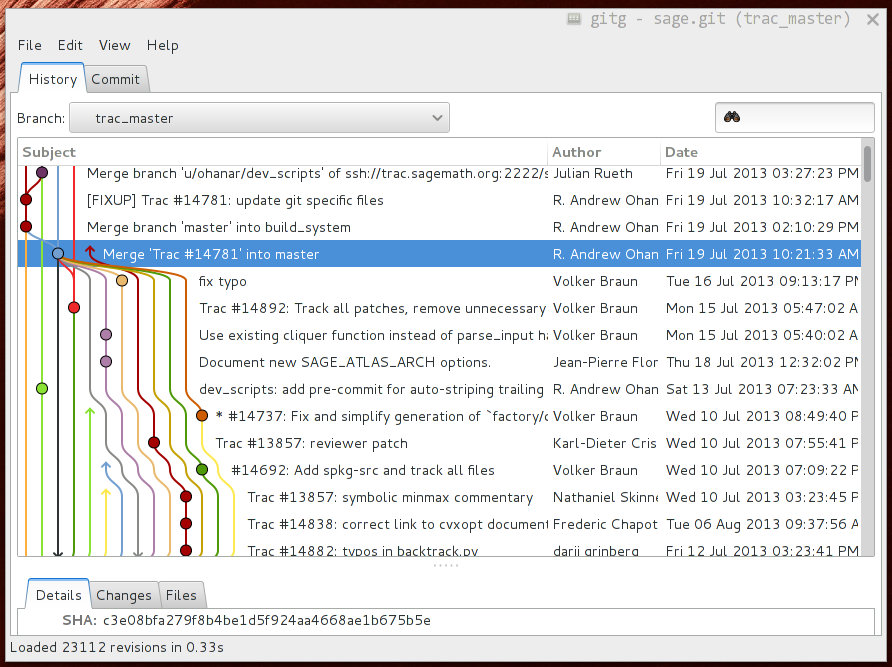
\includegraphics[width=\paperwidth]{images/gitg_screenshot}}
  \begin{frame}[plain]
    % 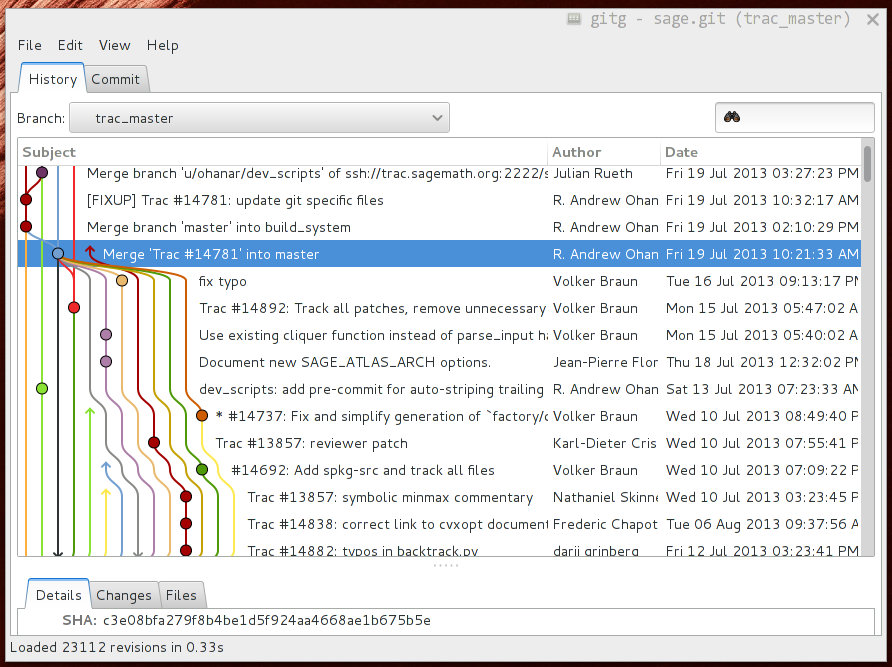
\includegraphics{images/gitg_screenshot}
  \end{frame}
}


\begin{frame}
  \frametitle{The Staging Area}

  Three places to store files:
  \begin{itemize}
  \item The git database (the \texttt{.git} directory)
  \item Staging area
  \item The working directory: all files outside of \texttt{.git} 
  \end{itemize}

  \begin{block}{Staging area}
    The staging area are the files that will be committed by
    \texttt{git commit}
    \begin{itemize}
    \item Show staging: \cmd{git status}
    \item Add to staging: \cmd{git add <filename>}
    \item Remove from staging: \cmd{git reset HEAD <filename>}
    \end{itemize}
  \end{block}
\end{frame}




\begin{frame}
  \frametitle{Committing Changes}

  \begin{block}{Creating a commit}
    \begin{itemize}
    \item 
      \cmd{git commit}
    \item Specify commit message on the command line:\\
      \cmd{git commit -m "my commit message"}
    \end{itemize}
  \end{block}
  
  Each commit is uniquely specified by the SHA1 hash\footnote{a 40
    digit hex number} of
  \begin{itemize}
  \item All changes to files
  \item All parent commits
  \item The commit message
  \end{itemize}
  None of these can ever be changed, including all direct and indirect
  parents.
\end{frame}


\begin{frame}
  \frametitle{Branches}

  Branches organize parallel development
  \begin{itemize}
  \item A branch is just a shortcut for a particular commit
  \item If you create a new commit, the branch automatically advances
    to it
  \item The default branch is \texttt{master}, but you can use any name
  \item \texttt{HEAD} is the commit at the tip of the branch:\\
    \cmd{git show HEAD}
  \item \texttt{HEAD$\sim$} is the parent of \texttt{HEAD}
  \item \texttt{HEAD$\sim$2} is the parent of the parent of
    \texttt{HEAD}
  \item etc.
  \end{itemize}
\end{frame}


\begin{frame}
  \frametitle{Remote Repositories}
  
  \begin{itemize}
  \item Remotes repositories are bookmarks.
  \item Configure with \cmd{git remote}
  \item \textbf{D}istributed VCS: all remotes are equal.
  \item The "important" one (to you) is usually called \texttt{origin}
  \end{itemize}

  If there are no conflicts:
  \begin{itemize}
  \item Upload your changes to the remote repository:\\
    \cmd{git push <remote>}
  \item Download changes from the remote repository and update the
    local working directory:\\
    \cmd{git pull <remote>}
  \item There is a default remote for each branch, see\\
    \cmd{git remote show <remote>}
  \end{itemize}

\end{frame}






%%% Local Variables:
%%% TeX-master: "talk"
%%% eval: (TeX-PDF-mode 1)
%%% End:
